% !TEX root = ../../../MathModel.tex
% 负责人：罗财能。
\subsubsection{模型求解}
\label{sec:q4:solution}

\textbf{（1）完整枚举与独立核验。}
对6个不可拆单元使用规范组号编码：首个单元属于第1组，后续单元只能加入已有组，或建立下一个新组，最终恰好出现$K$个组号。
该编码消除仅交换组名造成的重复，不删去任何实质不同的分组。
无标签非空分区数满足第二类Stirling数递推
\begin{equation}
  S(n,K)=K S(n-1,K)+S(n-1,K-1),
  \qquad S(6,2)=31,\quad S(6,3)=90.
  \label{eq:q4:enumeration}
\end{equation}
边界为$S(0,0)=1$，$S(n,0)=0$（$n>0$），$S(n,K)=0$（$K>n$）。
对每个候选计算各类占用峰值、分类库存缺口与工作量，再按式\eqref{eq:q4:objective}排序。
对选中方案和均衡对照进一步生成达到资源峰值下界的实体分配。

独立验证器从第三题原方案重新构造任务、依赖及充电区间，枚举全部带标签分配后去重，核对候选完整性。
资源峰值则直接在各任务开始时刻统计活动区间，不复用求解器的事件扫描算法。
最终11\,280项检查全部通过，另有12项测试覆盖端点衔接、微小真实重叠、充电导致的额外电池需求，以及分组或资源分配被改动时的拒绝行为。
本次计算得到的31个两组候选、90个三组候选均存在库存缺口，故在本文口径下，现有库存不能支持所要求的独立分组执行。

\textbf{（2）资源优先分区与配置。}
两组方案为：G1包含除S004外的14个服务区，G2仅包含S004。
三组方案为：G1包含除S004、S006外的13个服务区，G2仅包含S004，G3仅包含S006。
具体工作量和资源配置分别见表\ref{tab:q4:group-work}和表\ref{tab:q4:group-resources}，空间点位见图\ref{fig:q4:partition}。
图中颜色仅表示任务归属，不代表额外设置的地理边界。

\begin{table}[htbp]
  \centering
  \caption{资源优先方案的任务分组与工作量}
  \label{tab:q4:group-work}
  \begin{tabular}{clrrr}
    \toprule
    方案／组 & 服务区 & 货箱数 & 质量（kg） & 工作量（min） \\
    \midrule
    两组G1 & 除S004外14区 & 74 & 699 & 1059.88 \\
    两组G2 & S004 & 6 & 59 & 71.92 \\
    \midrule
    三组G1 & 除S004、S006外13区 & 68 & 640 & 995.99 \\
    三组G2 & S004 & 6 & 59 & 71.92 \\
    三组G3 & S006 & 6 & 59 & 63.90 \\
    \bottomrule
  \end{tabular}
\end{table}

\begin{table}[htbp]
  \centering
  \caption{资源优先方案各组最低配置；向量顺序均为A、B、C型}
  \label{tab:q4:group-resources}
  \begin{tabular}{lcccc}
    \toprule
    方案／组 & 运输机（架） & 电池（组） & 中继机（架） & 能源组件（组） \\
    \midrule
    两组G1 & $(4,2,2)$ & $(6,4,3)$ & 2 & 3 \\
    两组G2 & $(0,0,1)$ & $(0,0,1)$ & 1 & 1 \\
    两组合计 & $(4,2,3)$ & $(6,4,4)$ & 3 & 4 \\
    \midrule
    三组G1 & $(4,2,2)$ & $(5,4,3)$ & 2 & 3 \\
    三组G2 & $(0,0,1)$ & $(0,0,1)$ & 1 & 1 \\
    三组G3 & $(1,1,0)$ & $(1,1,0)$ & 0 & 0 \\
    三组合计 & $(5,3,3)$ & $(6,5,4)$ & 3 & 4 \\
    \bottomrule
  \end{tabular}
\end{table}

两组共需9架运输机、14组运输电池、3架中继机和4组能源组件，合计30件。
其中C型运输机、中继机各缺1架；2组能源组件虽有余量，但无法替代缺少的机体。
与27件的共享池下界相比，多需1架C型运输机、1组C型电池和1架中继机，共增加3件，增幅为11.11\%。
新增C型电池可以由现有库存承担，因此分组额外配置3件与库存缺口2件并不矛盾。

三组共需11架运输机、15组运输电池、3架中继机和4组能源组件，合计33件。
相对于现有库存，A、B、C型运输机各缺1架，中继机缺1架，B型电池缺1组，共缺5件；能源组件仍余2组。
相对于共享池，增加A、B、C型运输机各1架、B和C型电池各1组、中继机1架，共增加6件，增幅为22.22\%。
分类需求与库存的对应关系见图\ref{fig:q4:resources}。

缺口的直接原因是任务隔离后失去组间错峰复用机会。
单独承担S004的组仍需要C型运输机及中继机，而其余组的相应峰值不能同步消失；再将S006单独成组，又增加A、B型机及B型电池的独立配置。
由于时刻已冻结，不能用推迟任务、调整中继保障或跨组借机消除这些缺口。
补足相应资源后，各组才可按给出的实体分配独立执行。

\textbf{（3）工作量均衡的代价。}
资源优先方案的工作量CV分别为0.872908和1.159683，说明工作集中在大组，三组方案的不均衡更明显。
这与C02不可拆单元有关：其含10个服务区、47个货箱，累计任务工作量718.72\,min，占全部1131.81\,min的63.50\%。
任何分区都必须把这些任务放入同一组，故不能仅靠细调其他5个单元实现接近均分。

为量化取舍，再采用先最小化$\operatorname{CV}_L$、再比较缺口与总配置的字典序。
两组均衡方案将C02单独成组，另5个单元组成另一组，工作量分别为718.72和413.09\,min。
三组均衡方案分别为$\{\mathrm{S001},\mathrm{S011}\}$、C02、
$\{\mathrm{S004},\mathrm{S006},\mathrm{S014}\}$，工作量分别为220.97、718.72和192.11\,min。
两种评价顺序的结果见表\ref{tab:q4:tradeoff}。

\begin{table}[htbp]
  \centering
  \caption{资源优先与均衡优先的比较}
  \label{tab:q4:tradeoff}
  \begin{tabular}{clrrrr}
    \toprule
    组数 & 评价顺序 & 总配置（件） & 缺口（件） & 工作量CV & 货箱数CV \\
    \midrule
    2 & 资源优先 & 30 & 2 & 0.872908 & 0.850000 \\
    2 & 均衡优先 & 45 & 16 & 0.270042 & 0.175000 \\
    3 & 资源优先 & 33 & 5 & 1.159683 & 1.096016 \\
    3 & 均衡优先 & 48 & 19 & 0.640737 & 0.541122 \\
    \bottomrule
  \end{tabular}
\end{table}

两组均衡方案的运输机、电池、中继机、组件配置依次为$(8,4,3)$、$(10,7,4)$、4、5；
三组均衡方案依次为$(9,5,3)$、$(10,8,4)$、4、5。
两者均比相应资源优先方案多需15件配置，库存缺口也均增加14件。
因此，更均衡的任务划分需要显著增加资源投入。
图\ref{fig:q4:tradeoff}展示全部候选及三指标帕累托集合；图中的二维投影仍以颜色保留缺口指标，不据投影位置单独判断支配关系。

\textbf{（4）方案选择与结果边界。}
若按式\eqref{eq:q4:objective}优先控制资源，两组方案更合适：相较三组，少需3件配置，库存缺口少3件，工作量CV也较低。
两种方案均保持原33个运输架次、8个中继架次和全部货箱交付时刻，联合返航完成时刻仍为161.37\,min，总能耗仍为80.686\,kWh。
此处能源指标沿用问题三任务能耗口径，不把新增闲置设备计为执行能耗。
在资源补足且模型假设不变的条件下，原硬期限、返航SOC和连续通信核验结果随固定任务一并保留；分组本身不会降低配送延迟或缩短救援时间。

计算脚本为\path{Group/Lcn/Code/run_q4.py}。
完整候选、逐架次独立资源编号及分区表保存于\path{Group/Lcn/Results/Q4/}。
文件\texttt{manifest.json}记录输入、代码与输出的校验指纹。
本文证明的是固定第三题方案、允许同型实体重新编号、不复制中继架次时的有限分区最优，不能推广为允许重排任务或改变通信保障后的全局最优。

\begin{figure}[!htbp]
  \centering
  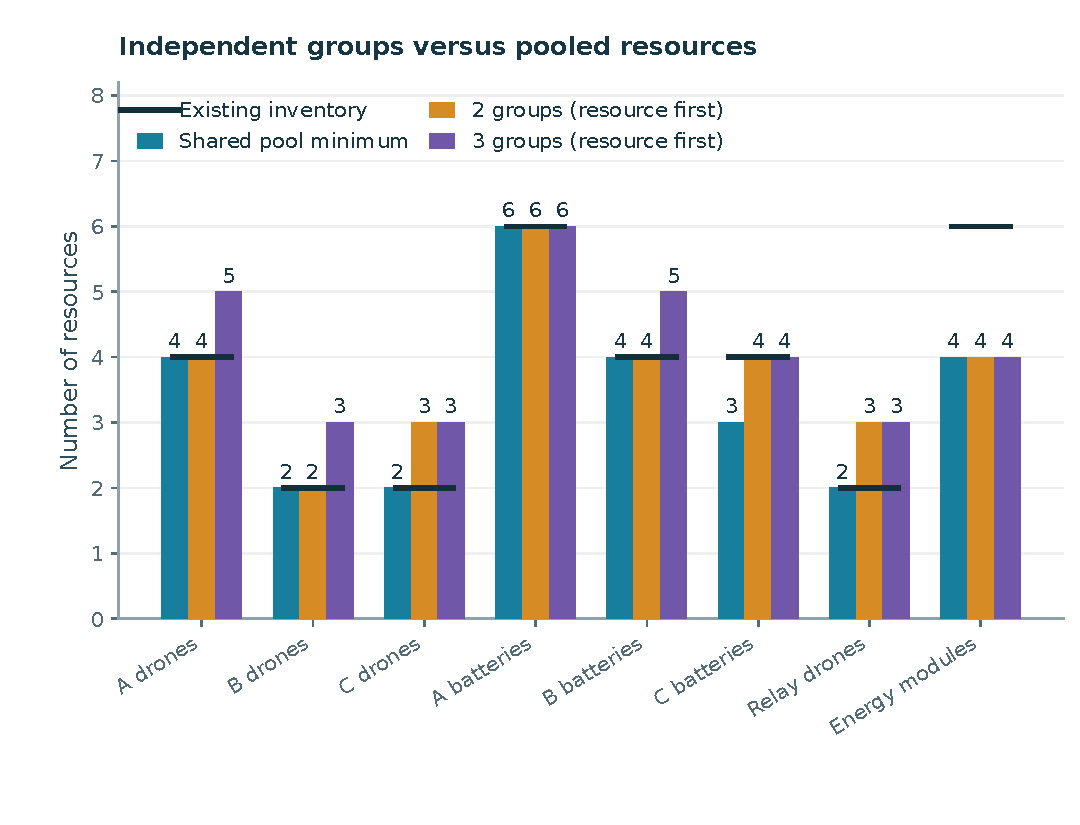
\includegraphics[width=0.98\textwidth,height=0.56\textheight,keepaspectratio]
    {../Results/Q4/02_resource_requirements.pdf}
  \caption{各类资源的共享池下界、独立分组需求及现有库存}
  \label{fig:q4:resources}
\end{figure}

\begin{figure}[p]
  \centering
  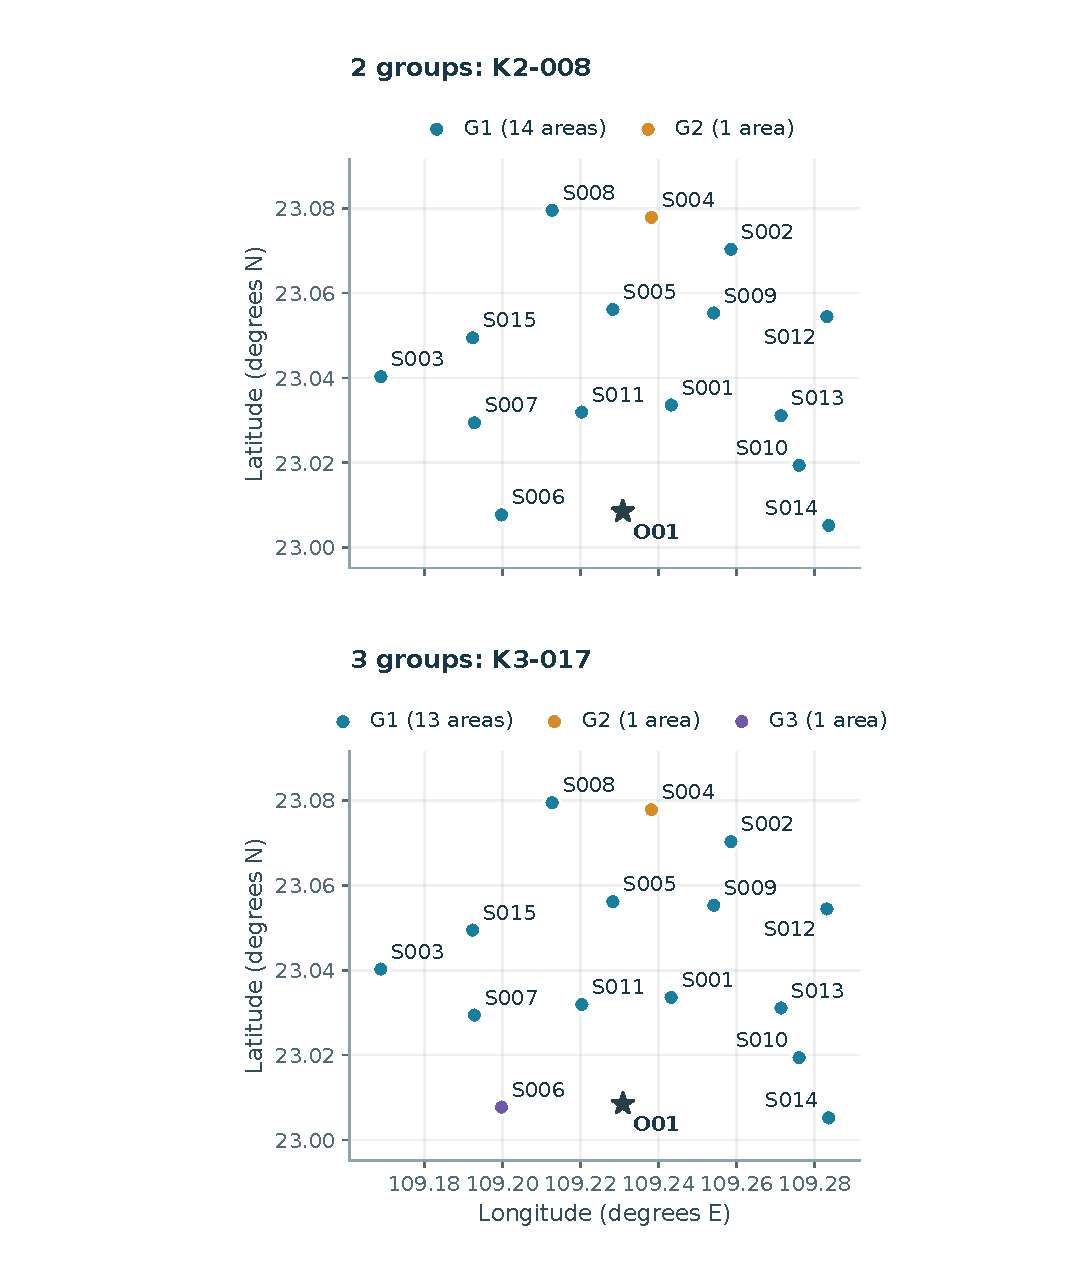
\includegraphics[width=0.98\textwidth,height=0.84\textheight,keepaspectratio]
    {../Results/Q4/01_partition_maps.pdf}
  \caption{资源优先的两组与三组方案；服务区按固定任务依赖分组}
  \label{fig:q4:partition}
\end{figure}

\begin{figure}[p]
  \centering
  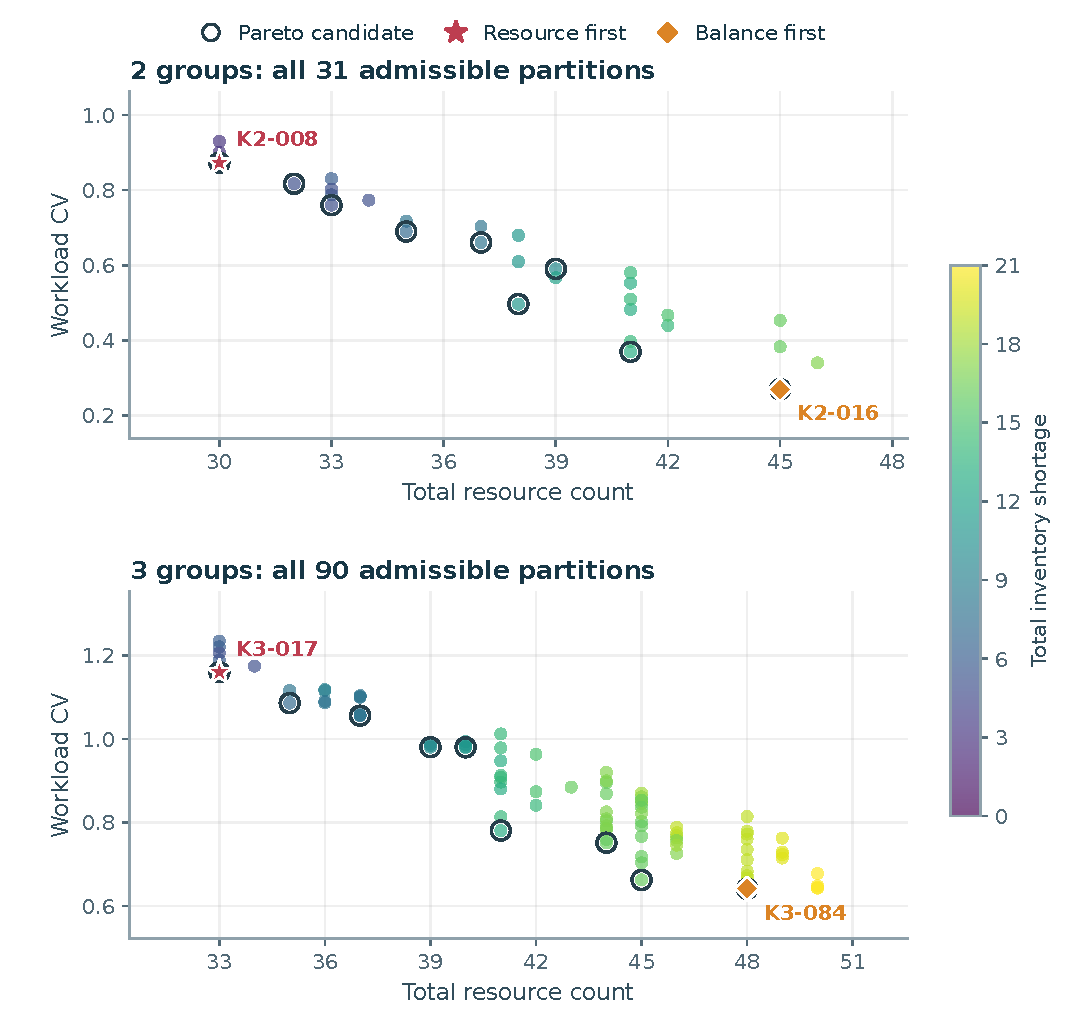
\includegraphics[width=0.98\textwidth,height=0.79\textheight,keepaspectratio]
    {../Results/Q4/03_tradeoff.pdf}
  \caption{全部31个两组与90个三组候选的资源、库存缺口和均衡权衡}
  \label{fig:q4:tradeoff}
\end{figure}

\clearpage
